\chapter{\textsc{PathObjects} for Squeak/Smalltalk}
\label{c:implementation}

\todo[inline]{Introduction}

\section{Prototypic Implementation}

%\begin{figure}
%	\centering
%	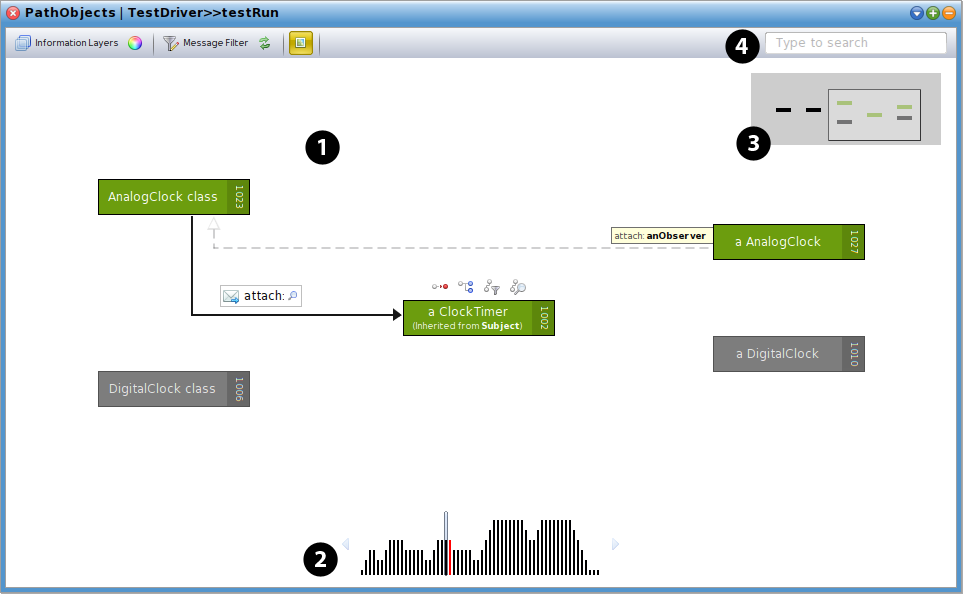
\includegraphics[width=1\textwidth]{../images/04-ImplMainWindow}
%	\caption[TOC Caption]{Foobar}
%	\label{fig:ImplementationMainWindow}
%\end{figure}

\subsection{Navigation}
\subsection{Exploration}
\subsection{Focusing}
\subsection{Information Layers}

\section{Data Acquisition}
This section describes how the data required for the reconstruction of object interactions is gathered.
The basic prerequisite is that objects can be distinguished and identified.
Since the Squeak image does not offer an adequate functionality, the strategy that was applied to solve this issue is depicted in Section \ref{ss:ImplementationTracingIdentification}.
Section \ref{ss:ImplementationTracingApproach} describes how the tracing approach works.
Finally, Section \ref{ss:ImplementationTracingReferences} shows how the tracking and mapping of outbound object pointers are implemented.

\subsection{Identification of Objects}
\label{ss:ImplementationTracingIdentification}
The fundamental requirement for the reconstruction of object interactions from traces is that object instances can be identified unambiguously.
Unfortunately, the Squeak image does not provide such a functionality out of the box.
Though objects do have an \inlinecode{identityHash} attribute, the value of this attribute is neither unique nor stable \cite{goldberg_smalltalk-80:_1983}.
In the virtual machine we used, it is derived from the least significant bits of the object pointer which is managed by the virtual machine and represents the object's address in main memory.
Hence, the value of the object pointer and thus the value of the \inlinecode{identityHash} are subject to change during garbage collection, which may cause objects to be moved in main memory.
Furthermore, since the \inlinecode{identityHash} uses only the 12 least significant bits, there is no guarantee that two objects that are not referentially equal cannot share a common hash value \cite{goldberg_smalltalk-80:_1983}.

The Squeak image does not offer a convenient way to access the object pointer, which could serve as unique identifier for objects.
There are workarounds that would allow to determine its value, but since this value still is subject to change during a tracing run due to the reasons pointed out above, it would require to disable garbage collection during this time span.
This could have undesired side effects, like excessive memory consumption or slow execution speeds due to increased memory allocation effort.

For these reasons, we chose a different approach that allows us to generate unique, stable identifiers for objects.
It exploits the fact that that a comparison for referential equality provided by the \inlinecode{==} method will always yield the correct result.
It returns true if the two objects have the same object pointer, and false otherwise.
Squeak provides a \inlinecode{WeakKeyIdentityDictionary} that has two beneficial properties for our use case.
First, it uses \inlinecode{==} comparison to test dictionary keys for equality.
That means that when using the objects that occur during tracing runs as keys, it is guaranteed that no two referentially distinct objects will be identified as the same key, and an object will always be mapped to the same key once it is present in the dictionary.
The second property is that it uses weak references to manage keys, which implicates that garbage collection of an object is not suspended by the fact that it is used as key in such a dictionary.

Consequently, this allows us to use objects occurring during tracing runs as keys, without interfering with the test execution.
Identifiers can be assigned to objects as values of the dictionary.
Thus, it is guaranteed that one object will always be mapped to the same identifier.
To ensure that no identifier is assigned to two referentially different objects, it is sufficient to use a continuously incrementing integer counter when assigning new identities, or respectively when adding new entries to the dictionary.

Since we presuppose that test cases are strictly deterministic (cf. Section \ref{s:DiscussionLimitations}), this strategy results in another benefit.
Namely, objects will always be assigned the same identifier in different tracing runs, since the identifier is only dependent on the chronological order in which objects occur in a trace.
In other words, to stick to the observer example, the instance of \inlinecode{DigitalClock} will always be assigned with the identifier \inlinecode{27} no matter how often the test is executed, since it is the 27th object that occurs in the trace.
This is an important property and prerequisite for the tracing and mapping of outbound object pointers (cf. Section \ref{ss:ImplementationTracingReferences}).

The current implementation constructs a new dictionary of identifiers for each test execution.
But it would also be possible to share identifiers of long living objects like classes across all tracing runs, if a global dictionary were used.
However, we are unaware of a use case that could exploit this possibility, and additional measures would be required to ensure the property described in the previous paragraph.
For these reasons, we favored trace-local over global identity generation.

\subsection{Tracing Approach}
\label{ss:ImplementationTracingApproach}
This section depicts the fundamental functional principles of the \textsc{PathTools} tracing framework that served as a basis of our prototypic implementation and describes the extensions that were required to adapt this framework to our requirements.

\subsubsection{Fundamental Functional Principles}

The fundamental idea behind the \textsc{PathTools} tracing approach is the distinction between shallow analysis and subsequent refinement runs.
During the shallow analysis phase, a trace of a selected test case is constructed that consists only of the bare minimum of information that is required for the reconstruction of the test execution.
This trace is presented to the developer who then can define which additional information is relevant for this specific scenario.
Refinements runs are performed to gather that additional information.
Thus, an extensive up-front collection of potentially useful information can be avoided. 

\begin{figure}[tb]
	\centering
	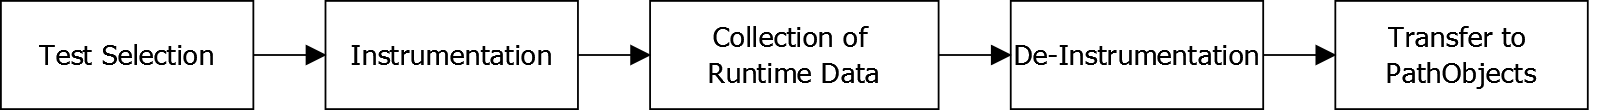
\includegraphics[width=0.9\textwidth]{../images/04-Tracing}
	\caption[TOC Caption]{Tracing foo}
	\label{fig:ImplementationTracing}
\end{figure}

\subsubsection{Shallow Analysis}

Figure \ref{fig:ImplementationTracing} depicts the fundamental steps that are performed by the \textsc{PathTools} tracing framework to generate an execution trace.
First, the user selects a test case of interest that should be traced and visualized.
For instance, this selection can be done through the list of test coverage information that is displayed next to methods in the source browser provided by the \textsc{PathTools} framework.
A \inlinecode{Tracer} object is generated which subsequently initiates the instrumentation phase.
Each method covered by the selected test case is replaced by a \inlinecode{MethodWrapper} that contains the fundamental tracing functionalities.
Thereby, only those methods are regarded that lie within the user-defined tracing scope, i.e. are a member of one of the packages the user selected for tracing.

Method wrappers \cite{brant_wrappers_1998} offer a convenient way to intercept the execution of specific methods.
As the name suggests, they wrap instances of \inlinecode{CompiledMethod} and take their place in the method dictionary of the corresponding class.
They can be utilized to execute code before and after the invocation of the wrapped method.
Furthermore, they allow the inspection and manipulation of arguments as well as of the return value of a message send.
Thereby, the operation of method wrappers is fully transparent for the callers of wrapped methods.

Afterwards, the tracer executes the specified test case.
Since all methods of interest are instrumented at this stage, they automatically report their execution to the tracer.
As method entry and exit events are recorded, a call tree of the selected test case can be constructed.

Once the execution of the test case finishes, the tracer triggers the de-instrumentation phase.
The previously created method wrappers are removed from the method dictionaries and the wrapped compiled methods are put back into their original places.

Finally, the collected information can be converted to a \textsc{PathObjects} trace, which resembles a sequential representation of the execution rather than a tree structure.

\subsubsection{Refinement Runs}
Conceptually, refinement runs are very similar to the shallow analysis process.
The differences are that no test case has to be selected, since the tracer already has a reference to the covered test case.
Furthermore, only those methods are instrumented that are actually required to collect the data that should be refined.
For instance, if the developer queries the state of an argument for a specific message send, only this method is instrumented.
Afterwards, the test is executed again and the installed method wrapper verifies if the current message send is the one the developer specified.
If this is the case, the state of this argument is recorded and reported to the tracer.
Once the test is finished, all method wrappers are removed, and the trace visualization can be updated with the refined information.

The fundamental prerequisite of this strategy is that test cases are strictly deterministic (cf. Section \ref{ss:DiscussionLimitationsTestQuality}).
Otherwise, the returned information might not be related to the developer's query.
For instance, the state of a different object might be returned when a method is called with different arguments in repeated executions.
Additionally, non-deterministic branching that yields a diverging call tree could have the consequence that the refinement run never reaches the specified point of the execution.

\subsubsection{Extensions}
In order to be suitable for the purposes of \textsc{PathObjects}, the tracing framework had to be extended in two places.
First, a custom \inlinecode{MethodWrapper} had to be implemented that collects the information required for the reconstruction of object interactions.
For each wrapped executed method, this specialized wrapper reports integer identifiers of the receiving object, of the method arguments, and of the return value to the tracer.
Thereby, argument objects are flattened.
That means that if collections of objects are used as arguments, the identifiers of the objects contained in a collection are reported in addition to the identifier of the collection object itself.
Note that an identifier for the sender of a message is not captured, since it would require the expensive operation of stack inspection.
However, this information can be easily reconstructed from the tree structure of the traces, since the sender of a message is identical to the parent element of a call node in the call tree.

The second extension that had to be made is the implementation of a custom \inlinecode{Tracer} that provides some functionality required by our method wrappers and for additional refinement runs.
It provides an implementation of our object identification approach (cf. Section \ref{ss:ImplementationTracingIdentification}) that is used by the method wrappers to generate unique and stable identifiers for objects that occur during tracing.
Furthermore, it provides entry points for the exploration of outbound object references, and is responsible for the execution of refinement runs that are necessary to collect this information (cf. Section \ref{ss:ImplementationTracingReferences}).

\subsection{Reference Tracing}
\label{ss:ImplementationTracingReferences}
Outbound object pointers - or in other words the set of objects a specific object references - can be determined with the help of  \inlinecode{Object>>outboundPointers}.
However, this method returns only the set of directly referenced objects.
For example, if an instance of \inlinecode{Subject} administers a collection of observers, it would return only the collection object itself, but not the observer objects contained in this collection.
Undoubtedly, this is the technically correct behavior.
But for our purposes it seems more suitable to return those indirectly referenced objects along with the actual references. 
More often than not, this is the actually relevant information for a developer.
Therefore, we decided to flatten the objects returned by \inlinecode{outboundPointers}, and generate identifiers as depicted in Section \ref{ss:ImplementationTracingIdentification} for the resulting objects.
Thus, objects that are wrapped in collections are included when a developer queries the outbound references of a specific object.

Unfortunately, the collection of object references is an expensive operation in two respects.
First, a call of \inlinecode{outboundPointers} is time consuming and thus could slow down the tracing process significantly.
Second, the amount of collected data could grow rapidly if all outbound pointers of all involved objects were collected up-front.
For these reasons, we decided to implement the tracking of object references with the help of refinement runs.
As soon as the user selects an object for reference tracing, the outbound pointers of this object are collected whenever the user steps to another part of of the execution history.
The respective referenced objects are highlighted with a user-defined background color.

As pointed out in Section \ref{ss:ImplementationTracingIdentification}, objects will always be associated with the same identifier in repeated test executions.
This fact is exploited to map the references that are returned from refinement runs to the objects of the current trace.
However, to guarantee that the identifiers from the refinement runs correspond to the identifiers from the shallow analysis run, both executions have to be identical in terms of the tracing code that is executed.
Hence, it is not sufficient to instrument only the method that represents the current step of the execution history.
It is important that the method wrappers request identifiers from the tracer in the exact same order and quantity as in the shallow analysis run.
For instance, if an object identifier would not be requested, all subsequent assigned identifiers would differ from the ones assigned during the first tracing run.
Therefore, the refinement runs for object reference tracing mostly correspond to a shallow analysis run.

\section{Visualization}
\subsection{Object Placement and Edge Routing}

This Section describes how \textsc{PathObjects} traces can be mapped to directed multigraphs and describes how we used the state of the art in graph drawing to place objects and messages in our interactive diagrams.
Furthermore, the interoperability of \textsc{Graphviz} and the Squeak environment is depicted.

\subsubsection{Preliminary Considerations}
The structure of a \textsc{PathObjects} trace can be interpreted as directed multigraph $G$, meaning that the edges constitute a multiset rather than a set (cf. Definition \ref{eq:ImplementationGraph}).

\begin{equation}
G = (V, E)
\label{eq:ImplementationGraph}
\end{equation}

Objects are the set of vertices $V$ in this graph.
Message sends between two objects form the multiset of ordered pairs $E$, with each element having the form $(S,R)$.
Thereby, $S$ denotes the sender of a message, and $R$ its receiver.
Contrarily to the traditional definition of simple directed graphs \cite{berge_graphs_1985}, loops have to be allowed, since message exchange between objects is bidirectional more than often.

The multiset $M \subseteq E$ of messages that are exchanged between two specific objects $n_1$ and $n_2$ can be expressed with the help of formula \ref{eq:ImplementationGraphMessages}.

\begin{equation}
M(n_1, n_2) = \left\{ (s,r) \in E \phantom{i}| \phantom{i} (n_1 = s \land n_2 = r) \lor (n_1 = r \land n_2 = s) \right\}
\label{eq:ImplementationGraphMessages}
\end{equation}

Consequently, this allows to express the number of messages $C_M$ that are exchanged between two objects as cardinality of $M$ (cf. Formula \ref{eq:ImplementationGraphMessageCardinality}).

\begin{equation}
C_M(n_1, n_2) = \left\vert \phantom{i} M(n_1, n_2) \phantom{i} \right\vert
\label{eq:ImplementationGraphMessageCardinality}
\end{equation}

The transformation of a \textsc{PathObjects} trace to a graph structure is straightforward.
All occurring objects are mapped one-to-one to vertices of the graph.
However, not all messages have to be represented by corresponding edges due to the fact that only a predefined number of messages $M_{max}$ are maximally shown in a diagram at the same time.
For instance, if $M_{max}$ is set to $4$, the graph that is presented to the user can never show more than $4$ edges between two objects, even if $5$ or more messages are exchanged between them.
Consequently, the number of edges $C_E$ that are required between two specific vertices is the minimum of the predefined maximum value $M_{max}$ and the number of messages that are actually exchanged between them.

\begin{equation}
C_E(n_1, n_2) = min(C_M(n_1, n_2),\phantom{i} M_{max})
\end{equation}

\subsubsection{Graph Drawing}

\subsubsection{Graphviz Integration}

\inlinecode{dot graph.dot -s100 -y -Tplain-ext -o graph2.dot}

\begin{graphviz}[caption={Foobar}]
digraph Observers {
	graph [rankdir=LR, splines=ortho]
	node [shape=none, fixedsize=true]
	edge [arrowhead=none];
	
	1002 [width=1.54, height=0.38, label="a ClockTimer"];
	1027 [width=1.61, height=0.38, label="a AnalogClock"];
	...
	1002 -> 1002;
	1002 -> 1027;
	1002 -> 1027;
	...
}
\end{graphviz}

\begin{graphviz}[caption={Foobar}]
graph 1 14.306 4.5451
node 1002 9.9444 3.1528 1.5417 0.375 "a ClockTimer" ...
node 1027 13.042 2.0139 1.6111 0.375 "a SDigitalClock" ...
...
edge 1002 1002 16 9.1735 3.255 8.6827 3.255 8.1389 3.255 ...
edge 1002 1027 7 9.8472 2.9659 9.8472 2.6371 9.8472 1.9896 ...
edge 1002 1027 7 10.719 3.2316 11.558 3.2316 12.778 3.2316 ...
...
stop
\end{graphviz}


\subsection{Information Layers}